
\chapter{Teamworking}

Super-languages are often used to process structured data in flexible
ways. The features provided by super-languages, such as pattern matching,
make it easy to process structured data. In addition, super-languages
are meta-aware and can reason about information in terms of its type.
This chapter shows how XMF can be used to process data that represents
information from different teams and how the high-level features can
process the information to detect inconsistencies in the data.

Modelling can be used to address large-scale business problems, where
teams of individuals collaborate to produce different parts of a model.
Teamworking raises the issue of model management: managing different
versions of a model and merging different versions into a single coherent
whole. Each team works independently on their version of the model.
The different versions must be compared for consistency. Inconsistencies
are identified and can be offered up for conflict resolution. Once
the versions are consistent then the approach allows them to be merged
into a single model.

The approach uses a meta-description of modelling data and therefore
does not depend on the language that has been used for modelling.
This is attractive because model comparison engines can be constructed
once and then used throughout an organisation.


\section{Overview}

%
\begin{figure}
\begin{center}

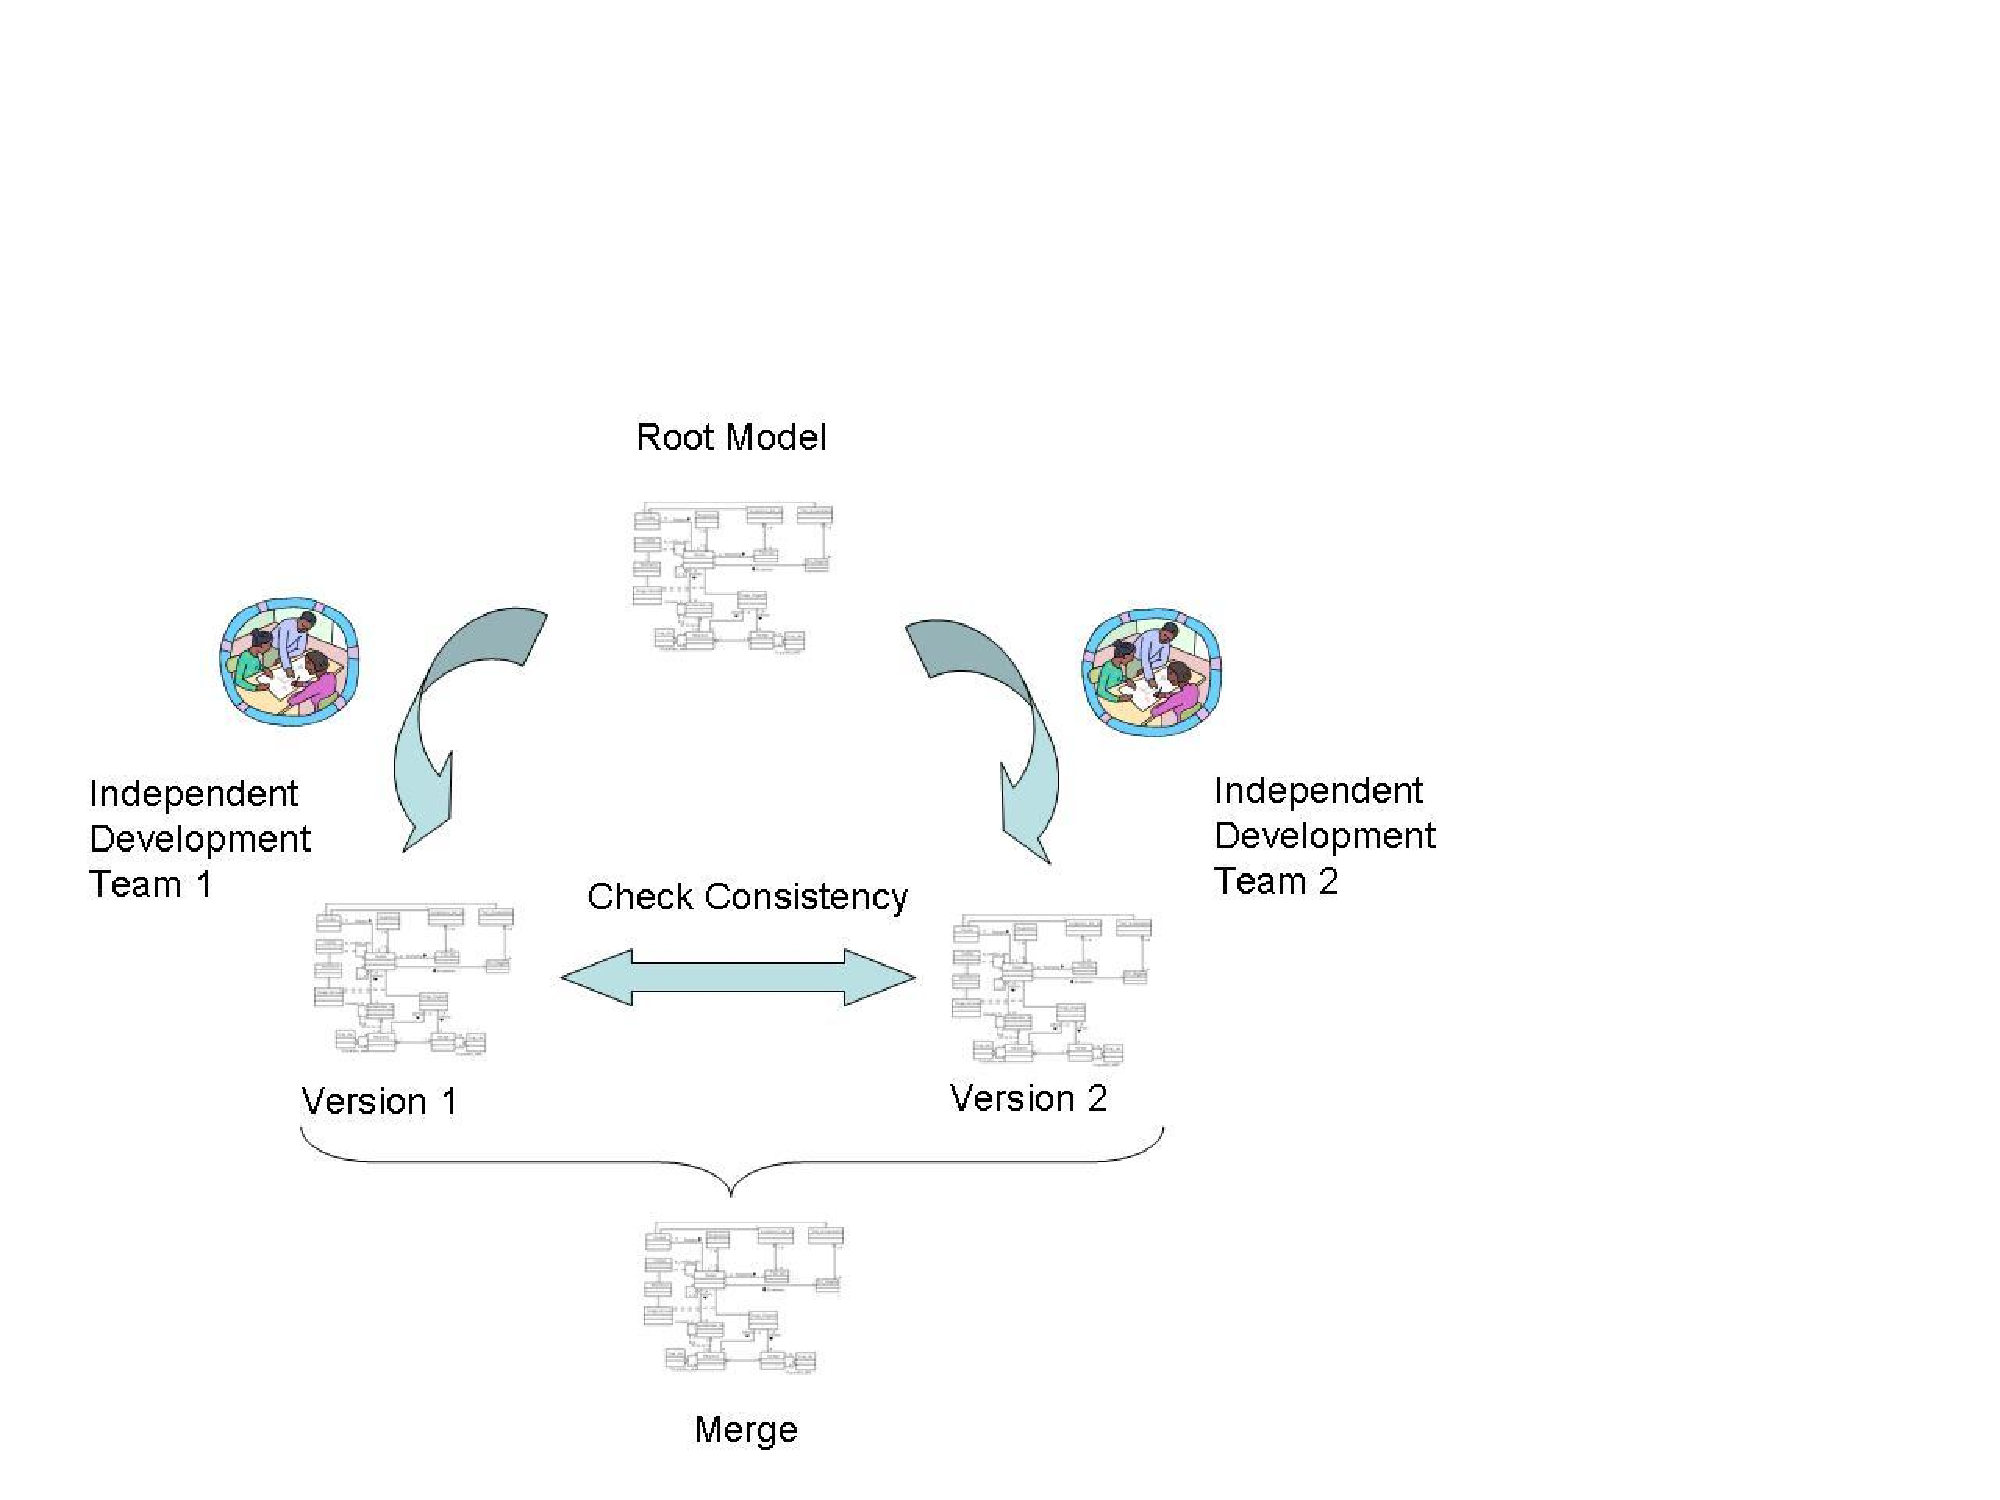
\includegraphics[width=12cm]{Programming/Teams/Images/Teamworking.pdf}

\caption{Overview Of Teamworking\label{fig:Overview-Of-Teamworking}}

\end{center}
\end{figure}


Systems that support teamworking, such as CVS and SVN provide functionality
that is shown in figure \ref{fig:Overview-Of-Teamworking}. A root
system is modified independently by two or more teams. The modifications
are referred to as \textit{deltas} leading to two or more new \textit{versions}. 

Once satisfied that their independent versions are OK, the teams want
to merge. To do this the versions must be compared for inconsistencies
which must be resolved. Inconsistencies may occur because each team
has modified an element in the root in a different way. Resolution
may involve one team changing their version so that it is consistent
with the other or may involve both teams removing the conflicting
parts.

Once the conflicts have been resolved, the versions can be merged
to provide a new baseline of the system. This process can be performed
any number of times and allows multiple teams to work concurrently
on a large system.

Conventional technologies for teamworking, such as CVS and SVN, work
with files. They compare the contents of the files on a character-and-line
basis. Conflicts arise when two versions of the same file have differing
changes at the same position.

Modelling technologies have a similar requirement to teamworking as
a file-content based approach. It is worth comparing the basic features
of the technologies, since the key aspects are similar whilst the
implementation details are different. When comparing files the following
features are important:

\begin{enumerate}
\item Files have unique identifiers: their names within the file-system.
These identifiers are used by the teamworking technology when comparing
files for potential conflicts, and when merging files.
\item Files have an internal structure: the lines and characters. The internal
structure of a file is used by the teamworking technology when comparing
files for potential conflicts. The internal structure is also used
when merging files.
\end{enumerate}
When comparing models similar features arise:

\begin{enumerate}
\item Model elements must have unique identifiers. These may be automatically
imposed by the system or may be supplied by the user. For example,
when a model element is created it may be tagged with the unique combination
of the user's details and the current time and date. Alternatively,
a naming scheme within the model may be used to uniquely identify
elements. In practice it may be necessary to use a combination of
system and user supplied identifiers.
\item Models have internal structure. At the meta-level, all model elements
are just objects with named slots. Conflicts arise when the same slot
of a uniquely tagged object is changed by both development teams.
Also, when merging models, changes to different slots of the same
object can be merged providing that it is uniquely tagged.
\end{enumerate}
%
\begin{figure}
\hfill{}\begin{lstlisting}
let counter = 0
in @Operation newTag()
     counter := counter + 1;
     counter
   end
end
  
@Class TaggedObject 
  @Attribute tag : Integer = newTag() (?,!) end
end
\end{lstlisting}\hfill{}

\caption{A Class for Uniquely Tagging Instances\label{fig:A-Class-for}}

\end{figure}


For the purposes of this technical note the tags will be automatically
generated for model elements. Figure \ref{fig:A-Class-for} shows
a class TaggedObject whose instances are uniquely tagged through the
use of an auxiliary operation newTag with local state 'counter'.

%
\begin{figure}
\begin{center}

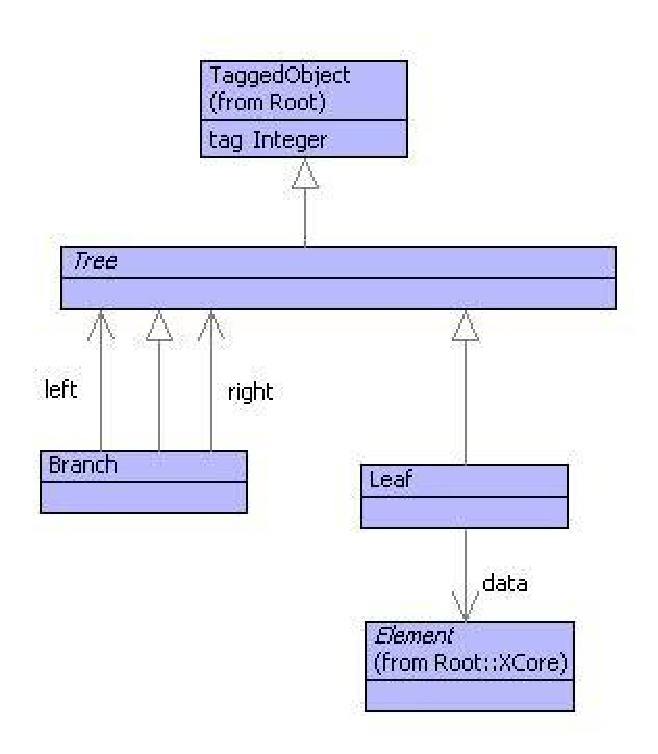
\includegraphics[width=12cm]{Programming/Teams/Images/Trees.pdf}

\caption{A Model of Binary Trees\label{fig:Binary Trees}}
\end{center}
\end{figure}


Example elements in this technical note are taken from the model shown
in figure \ref{fig:Binary Trees}. As noted above, model elements
are just objects. Provided that they are uniquely tagged and the structure
of the data is known, model-based teamworking technology can be applied
to any model. The example data forms binary trees where the elements
are all uniquely tagged and the leaves of the tree have arbitrary
data elements attached to them.

%
\begin{figure}
\begin{center}


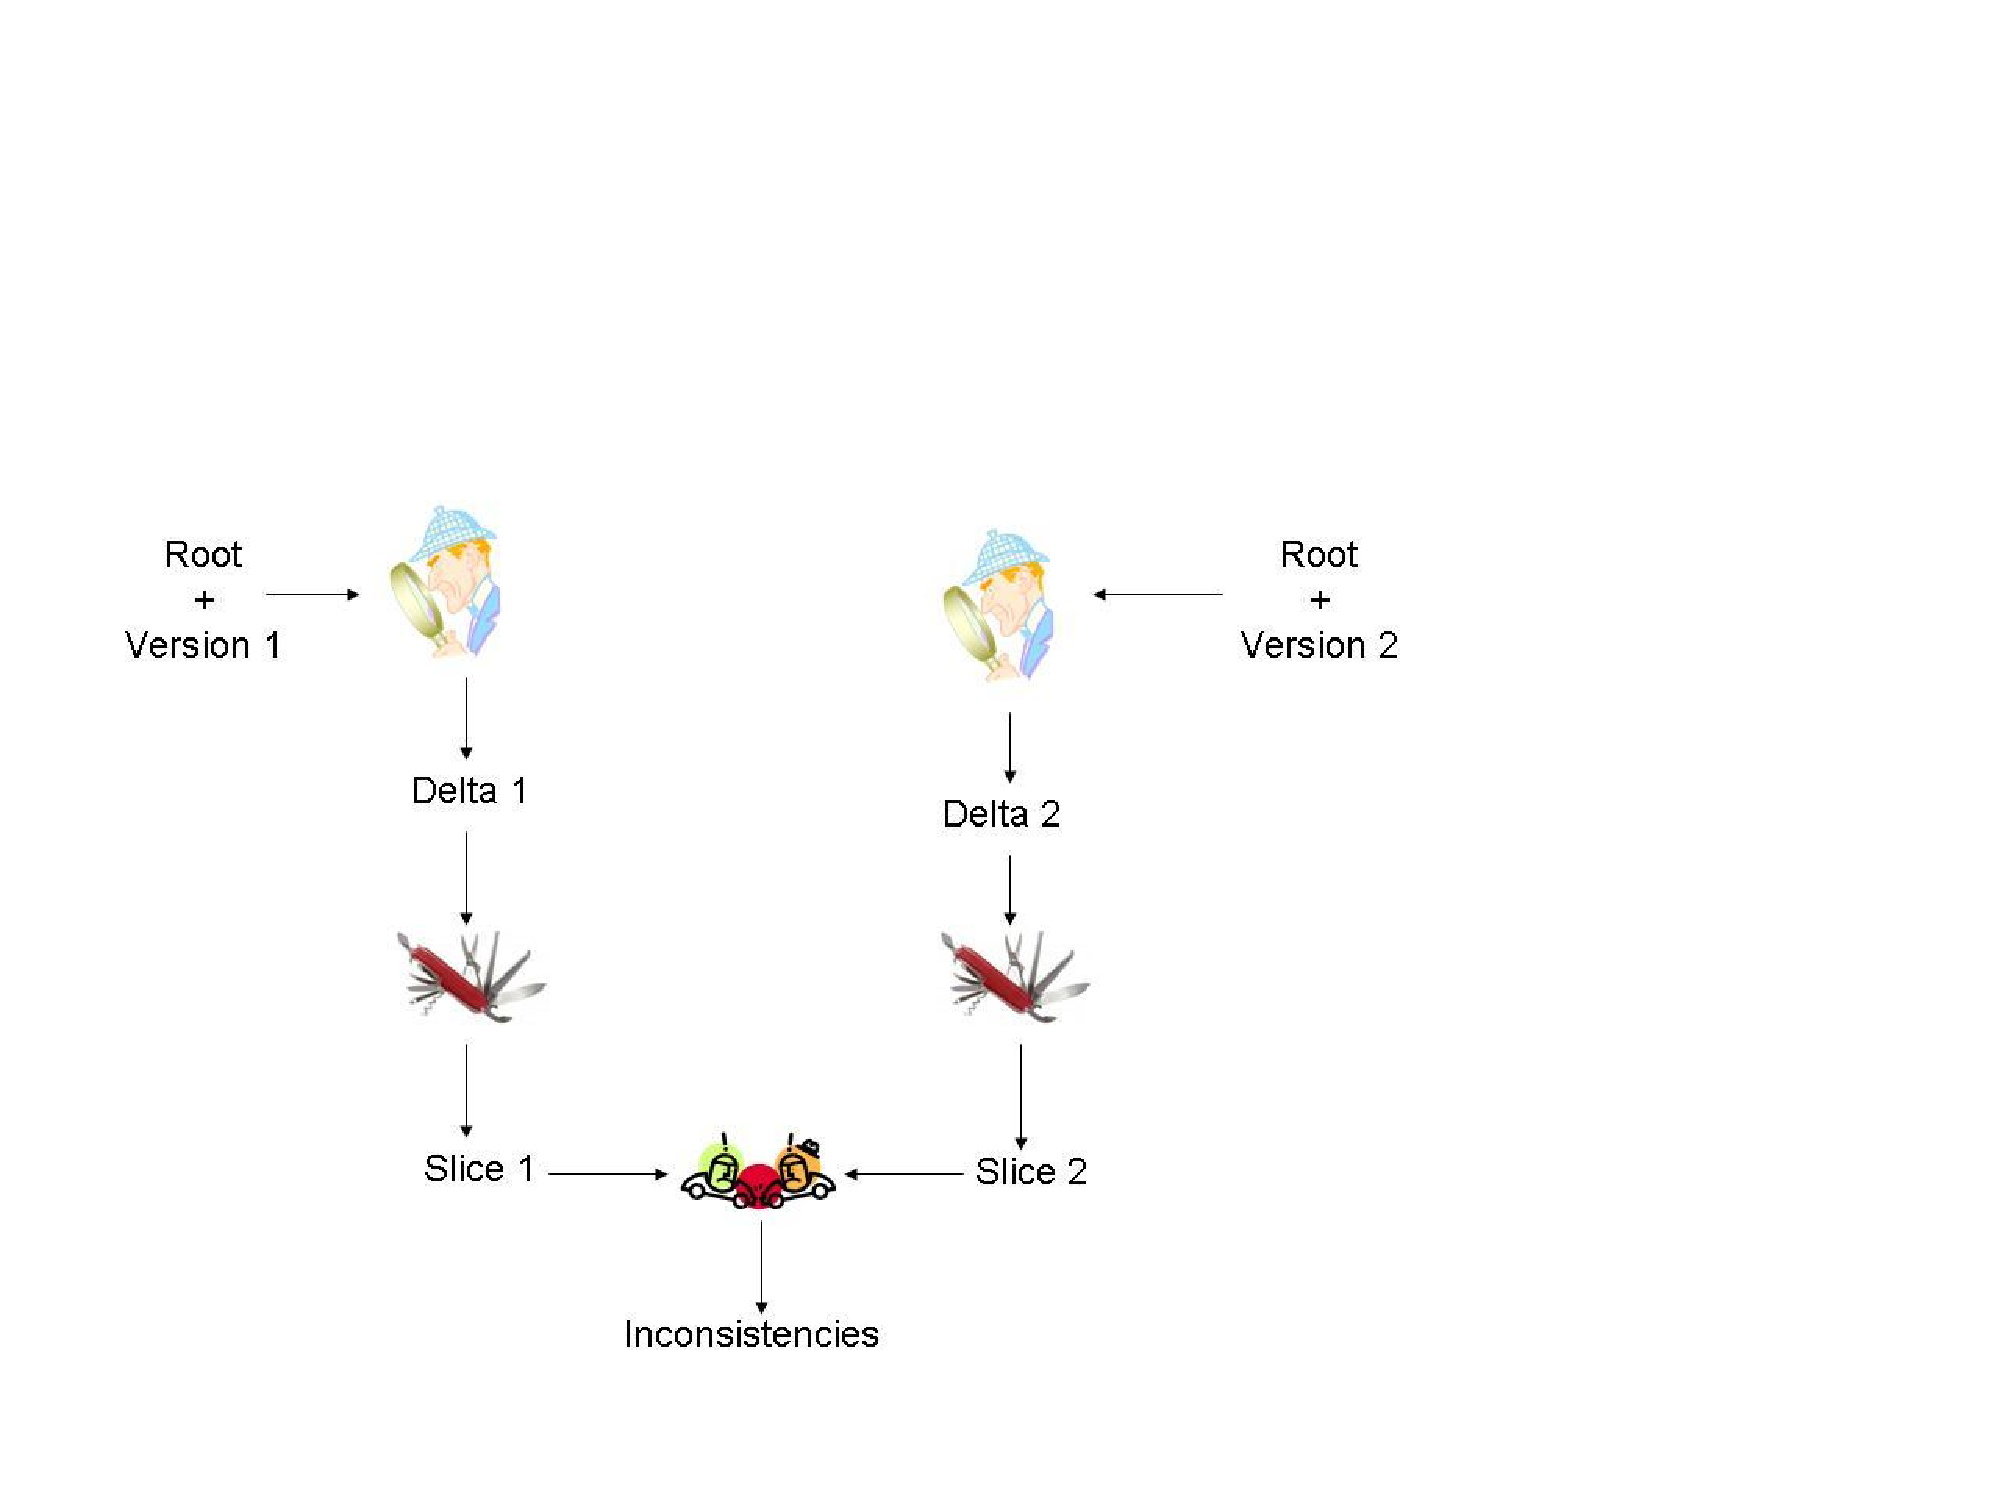
\includegraphics[width=12cm]{Programming/Teams/Images/Process.pdf}

\caption{Overview of Teamworking Implementation\label{fig:Overview-of-Teamworking}}

\end{center}
\end{figure}



\section{Overview of the Proposed Approach}

Figure \ref{fig:Overview-of-Teamworking} shows an overview of the
proposed tool support for teamworking. Both teams produce a new version
from the root. The root and version are compared and produce deltas.
Applying the delta to the root produces the version. The root can
be sliced with respect to the delta to produce just those model elements
that have changed. Two slices can be compared to see if the changes
are compatible; any incompatible changes are produced as inconsistencies.

If the two versions produce inconsistencies then they must be rationalized.
An inconsistency involves an element from each version and the slot
that has been modified. An inconsistency is rationalized when one
of the modifications (or both) is removed from the corresponding delta.
Once removed, the process is performed again, producing fewer inconsistencies.

The rationalization process continues until no inconsistencies arise.
In this case the deltas are independent and can be performed in any
order to produce a final merged model.


\section{The Delta Machine}

%
\begin{figure}
\begin{center}

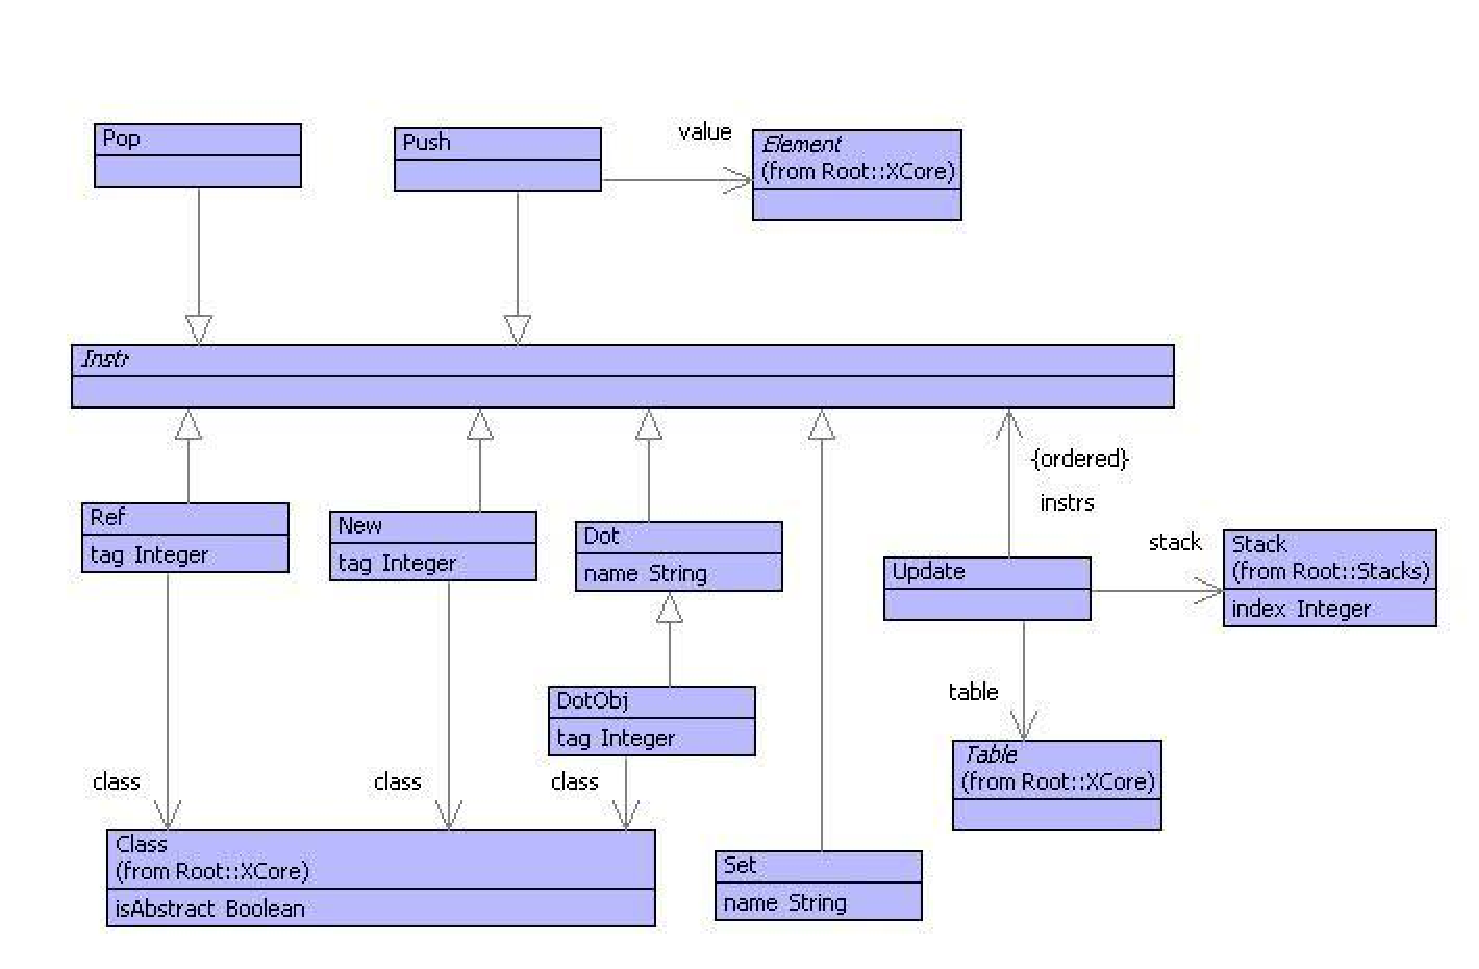
\includegraphics[width=12cm]{Programming/Teams/Images/Delta.pdf}

\caption{The Delta Machine\label{fig:The-Delta-Model}}

\end{center}
\end{figure}


Teamworking produces two or more versions based on a shared root.
Each version adds new elements and makes modifications to the root.
Large parts of the root will be left unchanged and can be ignored
when the versions are compared and merged. It is therefore useful
to be able to isolate the changes or \textit{deltas} that have been
applied by each team to the shared root. This section describes a
language and its execution engine used to model deltas.

Model elements are uniquely tagged objects. An object consists of
slots; each slot has a name and a value. A value is either atomic
(such as an integer or a string) or is an object. Models are arranged
as graphs where the nodes in the graph are values and the edges are
slots. A model-graph may have cycles, i.e. an object can refer directly
or indirectly to itself.

A delta is a modification to a model. A delta can change a slot value.
The new value may be atomic, may introduce a reference to an existing
object or may create a completely new object. Imagine a machine that
takes as input a model and a delta and \textit{runs} the delta producing
a new model. The delta machine is shown in figure \ref{fig:The-Delta-Model}.
A delta is a sequence of instructions, the machine is defined by a
class called Update.

%
\begin{figure}
\hfill{}\begin{lstlisting}
@Operation run1(instr)
    @Case instr of
(1)   Push(v) do
        stack.push(v)
      end
(2)   Pop() do
        stack.pop()
      end
(3)   Dot(n) do
        stack.push(stack.top().get(n))
      end
(4)   Set(n) do
        stack.top().set(n,stack.pop())
      end
(5)   Ref(c,i) do
        stack.push(table.get(i))
      end
(6)   New(c,i) do
        let o = c()
        in o.setTag(i);
           table.put(i,o);
           stack.push(o)
        end
      end
      else self.error("Unknown instr: " + instr.toString())
    end
end
\end{lstlisting}\hfill{}

\caption{The Delta Machine Interpreter\label{fig:The-Delta-Machine}}

\end{figure}


The delta machine execution engine is defined in figure \ref{fig:The-Delta-Machine}.
The machine has a stack, used to hold for intermediate results and
the model being updated. The machine also has a table associating
the tags in the model with the model elements, used to move elements
around the model. To run the machine, the root model element is pushed
onto the stack, the table is populated with all associations in the
model and sequence of instructions is loaded onto the machine.

The machine executes by case analysis on the instructions. Each instruction
is popped from the instruction stack and performed by the operation
run1. Case (1) pushes an atomic value v onto the stack. Case (2) pops
the value at the head of the stack. Case (3) expects an object at
the head of the stack and pushes the value of slot n onto the stack.
Case (4) expects a value above an object on the stack. The value is
popped and the slot named n is updated. Case (5) pushes an existing
element in the model (held in the table) onto the stack. Case (6)
creates a new object of type c with tag i and pushes it onto the stack.

%
\begin{figure}
\subfigure[Tree Before Update]{

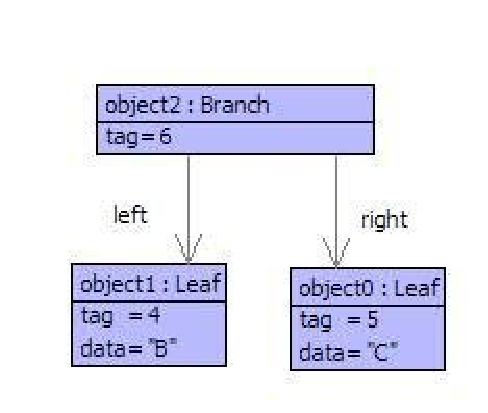
\includegraphics[width=12cm]{Programming/Teams/Images/Snapshot1a.pdf}}

\subfigure[Tree After Update]{

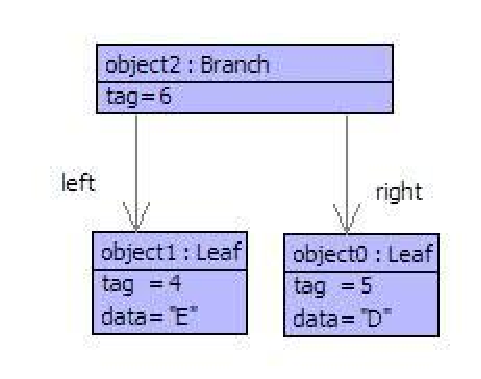
\includegraphics[width=12cm]{Programming/Teams/Images/Snapshot1b.pdf}}

\caption{Tree Update\label{fig:Tree-Update}}

\end{figure}


Figure \ref{fig:Tree-Update} shows a tree before and after modification.
The delta machine instructions that perform the change are as follows:

\begin{lstlisting}
Dot(left)
Dot(data)
Pop()
Push(E)
Set(data)
Set(left)
Dot(right)
Dot(data)
Pop()
Push(D)
Set(data)
Set(right)
\end{lstlisting}The delta machine program above runs by navigating from the root using
the Dot instructions. Each slot is referenced, its value is pushed
and then the slot is set. The delta machine program is produced by
a model comparator as described in the next section. The instructions
can be optimized by omitting redundant navigations:

\begin{lstlisting}
Dot(left)
Push(E)
Set(data)
Set(left)
Dot(right)
Push(D)
Set(data)
Set(right)
\end{lstlisting}
\section{Model Comparison}

Teamworking involves a root model and two or more versions. Given
a root and a version, a delta is a machine program that is produced
by comparing the root and version. The result is a machine program
that captures exactly the steps necessary to transform the root into
the version. This section describes a model comparator that is used
to produce a delta.

%
\begin{figure}
\hfill{}\begin{lstlisting}
@Operation compareObjects(new,old,oldDB,compared)
  if tag(new) = tag(old)
  then 
    if compared.hasKey(tag(new)) 
    then Seq{}
    else 
      compared.put(tag(new),tag(old));
      compareSlots(slots(new),slots(old),oldDB,compared)
    end
  elseif oldDB.hasKey(tag(new))
  then 
    let oldSlots = slots(oldDB.get(tag(new)))
    in Seq{Pop(),Ref(new.of(),tag(new))} + 
         compareSlots(slots(new),oldSlots,oldDB,compared)
    end
  else Seq{Pop()} + newObject(new,oldDB,compared)
  end
end
\end{lstlisting}\hfill{}

\caption{Object Comparison\label{fig:Object-Comparison}}

\end{figure}


Consider the models shown in figure \ref{fig:Tree-Update}. Suppose
that the before model is the root and the after model is a version
produced in a teamworking scenario. What steps are necessary to produce
the delta that transforms the root into the increment?

Starting with the root element of both models, compare the objects.
They both have the same tag and therefore at this stage no changes
have taken place. Now compare slots from each object. Start with the
left slot: traverse the slot, emit a Dot instruction, compare the
values found there, and emit a Set instruction. At this stage the
delta is:

\begin{lstlisting}
Dot(left),...,Set(left),...
\end{lstlisting}The values are both Leaf objects with the same tag. Therefore, compare
the data slot values: emit a Dot and a Set as before:

\begin{lstlisting}
Dot(left),Dot(data),...,Set(data),Set(left),...
\end{lstlisting}When the data slot values are compared, it is found that the value
has changed to E. Therefore emit a Pop instruction and Push the new
value:

\begin{lstlisting}
Dot(left),Dot(data),Pop(),Push(E),Set(data),Set(left),...
\end{lstlisting}If this is repeated for the right slot then the complete delta is
produced as shown in the previous section.

Figure \ref{fig:Object-Comparison} shows the operation which is the
entry point for the object comparison. The four arguments are: the
new object (initially the root element of the new version); the old
object (initially the root element of the root model) ; a table (oldDB)
associating tags with elements from the root model; and, a table (compared)
that records comparisons as they are performed so that the any comparison
happens once (otherwise cycles in the model would lead to cycles in
the comparator).

The second part of the operation shown in figure \ref{fig:Object-Comparison}
has not been covered by the running example. If the tags of the new
and old objects are not the same then this means that the old object
has been replaced with the new object. In this case, either some existing
element from the root model has been linked into the model, or the
new model contains a completely new object. This is determined using
the oldDB which contains associations for all the tags in the root
model.

%
\begin{figure}
\hfill{}\begin{lstlisting}
@Operation compareSlots(newSlots,oldSlots,oldDB,compared)
  if newSlots->isEmpty
  then Seq{}
  else
    let newSlot = newSlots->head then
        name = slotName(newSlot)
    in @Find(oldSlot,oldSlots)
         when slotName(oldSlot) = name
         do let newSlots = newSlots->tail;
                oldSlots = oldSlots->excluding(oldSlot)
            in compareSlot(newSlot,oldSlot,oldDB,compared) +
               compareSlots(newSlots,oldSlots,oldDB,compared)
       end
    end
  end
end
\end{lstlisting}\hfill{}

\caption{Slot Comparison\label{fig:Slot-Comparison}}

\end{figure}


Slot comparison is defined by the operation in figure \ref{fig:Slot-Comparison}.
The compareSlots operation simply runs through the new slots, finding
old slots with the same name and comparing them using the operation
compareSlot.

%
\begin{figure}
\hfill{}\begin{lstlisting}
@Operation compareSlot(newSlot,oldSlot,oldDB,compared)
  let name = slotName(newSlot);
      newValue = slotValue(newSlot);
      oldValue = slotValue(oldSlot)
  in if newValue.isReallyKindOf(Object)
     then 
       Seq{DotObj(name,value.of(),tag(newValue))} + 
         compareObjects(newValue,oldValue,oldDB,compared) + 
       Seq{Set(name)}
     else 
       Seq{Dot(name)} + 
         compareValues(value,oldValue,oldDB,compared) + 
       Seq{Set(name)}
     end
  end
end
\end{lstlisting}\hfill{}

\caption{Comparing Slot Values\label{fig:Comparing-Slot-Values}}

\end{figure}


Comparing slot values is shown in figure \ref{fig:Comparing-Slot-Values}.
This operation produces the Dot ... Set machine instructions. For
reasons to be explained later, if the slot values are objects then
a DotObj instruction is used.

%
\begin{figure}
\hfill{}\begin{lstlisting}
@Operation newObject(new,oldDB,compared)
  if compared.hasKey(tag(new))
  then Seq{Ref(new.of(),tag(new))}
  else 
    compared.put(tag(new),null);
    Seq{New(new.of(),tag(new))} +
      newSlots(slots(new),oldDB,compared)
  end
end
\end{lstlisting}\hfill{}

\caption{Creation of New Object\label{fig:Creation-of-New}}

\end{figure}


Figure \ref{fig:Creation-of-New} shows the instructions produced
when a slot in the new model contains an object that does not match
that in the old model. If the object has been encountered before then
a Ref instruction is produced (the machine will push a reference to
an existing object). Otherwise, the new object has not been seen before,
it is recorded and newSlots is used to process the slot of the new
object.

%
\begin{figure}
\hfill{}\begin{lstlisting}
@Operation newSlots(slots,oldDB,compared)      
  if slots->isEmpty
  then Seq{}
  else 
    let slot = slots->head
    in newSlot(slot,oldDB,compared) +
       newSlots(slots->tail,oldDB,compared)
    end
  end
end
  
@Operation newSlot(slot,oldDB,compared)
  if value.isReallyKindOf(Object)
  then 
    if oldDB.hasKey(tag(slotValue(slot)))
    then 
     Seq{Ref(slotValue(slot).of(),tag(slotValue(slot)))} +
      compareObjects(new,oldDB.get(tag(new)),oldDB,compared)
    else newObject(slotValue(slot),oldDB,compared)
    end
  else Seq{Push(slotValue(slot))}
  end +
  Seq{Set(slotName(slot))}
end
\end{lstlisting}\hfill{}

\caption{Checking Slots of a New Object\label{fig:Checking-Slots-of}}

\end{figure}


Checking new slots is defined in figure \ref{fig:Checking-Slots-of}.
Each of the new sots is inspected in turn; the job of newSlots is
to emit instructions that will initialize the slots of the newly created
object at the head of the machine stack.

If the slot value is an object that also occurs in the old model then
a Ref instruction is emitted and the two objects are compared. Otherwise,
if the value is an object it must be new, so further instructions
are produced by newObject. Otherwise the value must be atomic so it
is simply pushed. In all cases the last instruction emitted is a Set
instruction to modify the newly created object at the head of the
machine stack.

%
\begin{figure}
\hfill{}\subfigure[Tree Before Update]{

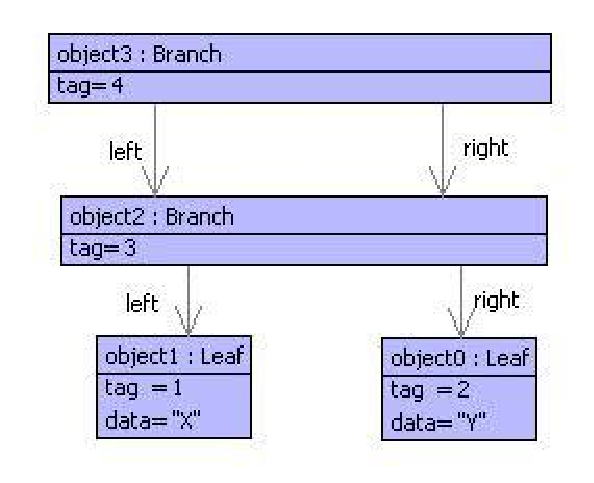
\includegraphics[width=12cm]{Programming/Teams/Images/Snapshot2a.pdf}}

\subfigure[Tree After Update]{

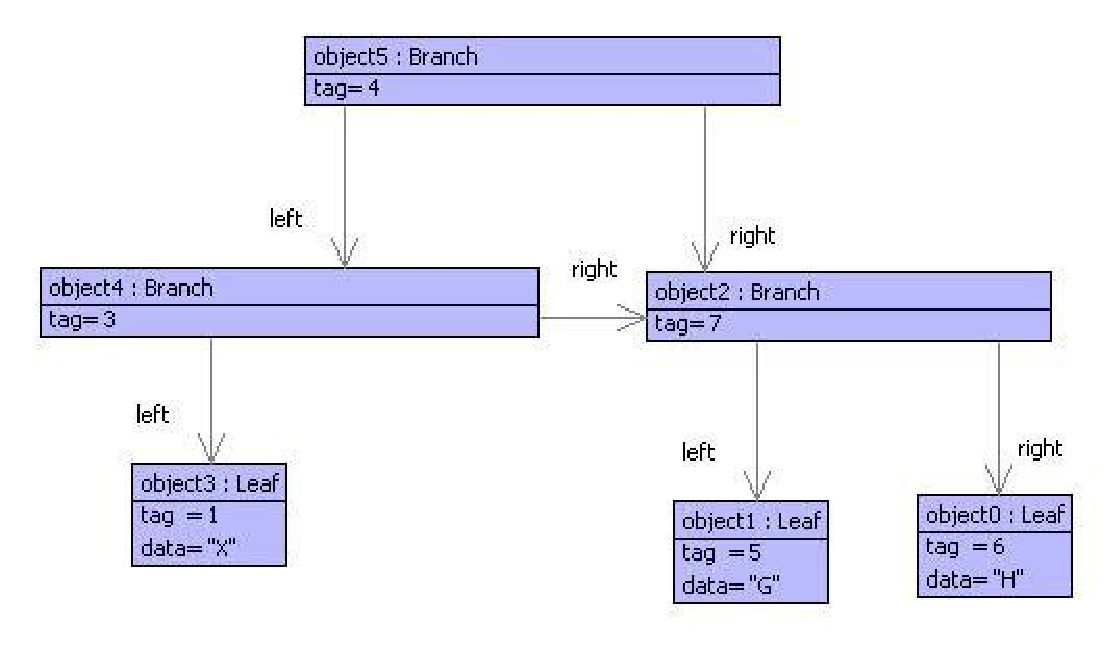
\includegraphics[width=12cm]{Programming/Teams/Images/Snapshot2b.pdf}}

\caption{A More Complex Tree Modification\label{fig:A-More-Complex}}

\end{figure}

Figure \ref{fig:A-More-Complex} shows a slightly more complex tree
modification in which a new branch is created and shared between two
different places in the tree. Comparison of the before and after states
produces the following delta:

\begin{lstlisting}
Dot(left)
New(<Class Branch>,14)
New(<Class Leaf>,12)
Push(G)
Set(data)
Set(left)
New(<Class Leaf>,13)
Push(H)
Set(data)
Set(right)
Set(right)
Set(left)
Ref(<Class Branch>,14)
Set(right)
\end{lstlisting}
\section{Model Slices}

Teamworking involves a root model and two or more version models.
The version models are produced by independent teams making modifications
to the same root model. Many of the elements in the root models may
be unchanged in the increments. When comparing the two versions for
consistency it is useful to be able to ignore the unchanged elements.
A model that describes just the changed elements in a version is called
a \textit{slice.} Two slices can be easily compared since they just
contain the elements that have changed. Two models are inconsistent
if the same elements have been changed in different ways; slices make
consistency checking easy. This section describes how to slice a model
with respect to a delta.

%
\begin{figure}
\begin{center}

\hfill{}\subfigure[Sliced Elements]{

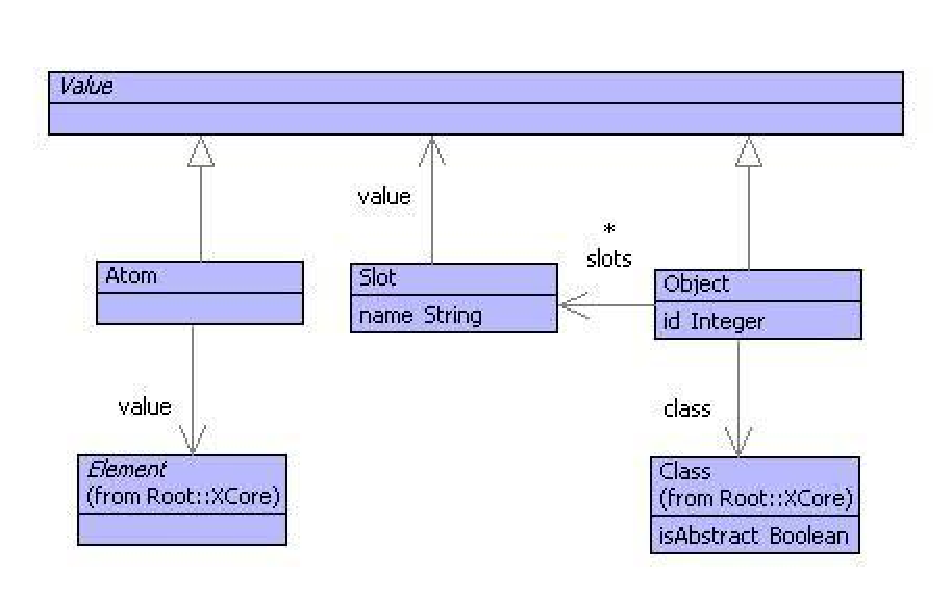
\includegraphics[width=12cm]{Programming/Teams/Images/Slice.pdf}}

\subfigure[Slicing Engine]{

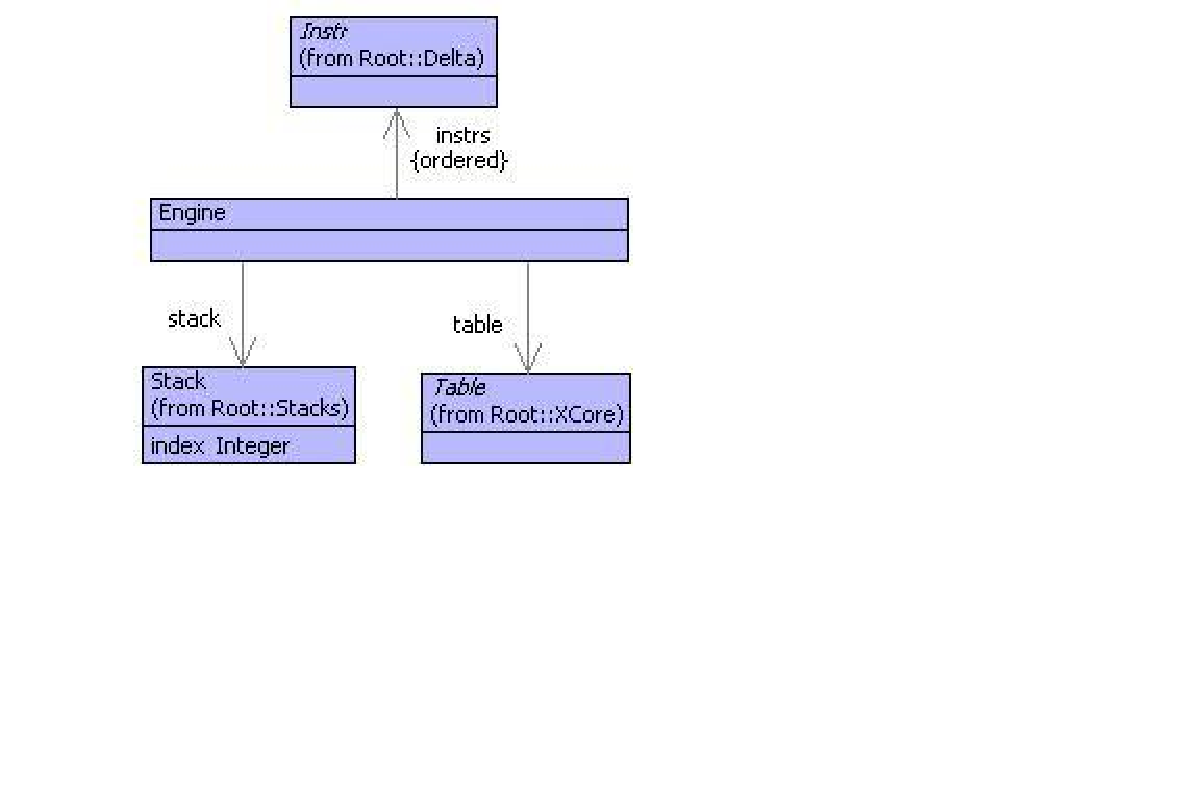
\includegraphics[width=12cm]{Programming/Teams/Images/SliceEngine.pdf}}

\caption{Model Slice\label{fig:Model-Slice}}

\end{center}
\end{figure}


Figure \ref{fig:Model-Slice} shows a model used to represent a slice.
Running a delta against a model using the slicing engine produces
a slice; the engine is like the delta machine except that it interprets
the delta instructions differently. To slice a model with respect
to a delta, the model is pushed onto the slicing engine, the delta
is loaded onto the machine and the instructions are performed. The
result at the head of the stack is an instance of the sliced object
model; only those things that are changed are contained in the slice.

%
\begin{figure}
\begin{center}

\hfill{}\begin{lstlisting}
@Operation slice(instr)
    @Case instr of
(1)   DotObj(n,c,i) do
        if table.hasKey(i)
        then stack.push(table.get(i))
        else
          let o = Object(c,i)
          in table.put(i,o);
             stack.push(o)
          end
        end
      end
(2)   New(c,i) do
        let o = Object(c,i)
        in stack.push(o);
           table.put(i,o)
        end
      end
(3)   Set(n) do
        let value = stack.pop() then
            obj = stack.top();
            slot = Slot(n,value)
        in obj.addToSlots(slot)
        end
      end
(4)   Push(v) do
        stack.push(Atom(v))
      end
      else self.error("Unknown instr: " + instr.toString())
    end
end
\end{lstlisting}\hfill{}

\caption{The Slicing Interpreter\label{fig:The-Slicing-Interpreter}}

\end{center}
\end{figure}


Figure \ref{fig:The-Slicing-Interpreter} defines the interpreter
that performs a single delta instruction on the slicing engine. If
the delta performs an update then the slicing engine records this
in the data model that is constructed at the head of the stack. It
is driven by case analysis on the instruction. Case (1) occurs when
an object slot is being referenced. In an optimized delta, slots that
contain objects are the only slots that need referencing (otherwise
they are being updated with atomic data and do not need referencing).
If the slot value has been seen before then the object data is in
the table, otherwise an object is created (recording that the object
is going to be updated) and recorded in the table.

Case (2) records the creation of a new object. Case (3) records the
update of a slot; the value is at the head of the stack. Case (4)
pushes some atomic data onto the stack ready for updating a slot.

%
\begin{figure}
\begin{center}

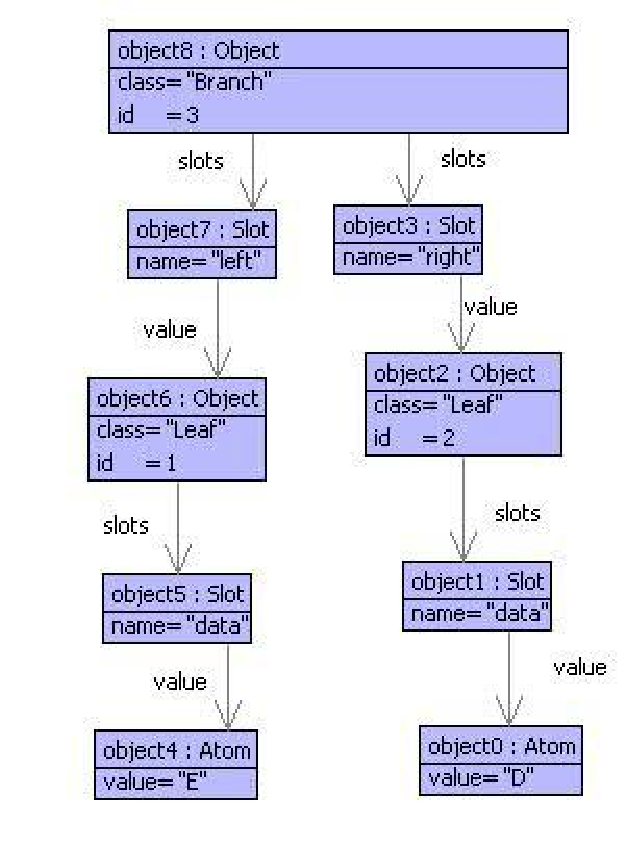
\includegraphics[width=12cm]{Programming/Teams/Images/SlicedSnapshot.pdf}

\caption{Model Slice\label{fig:SlicedModel}}

\end{center}
\end{figure}


Figure \ref{fig:SlicedModel} shows a slice created by running the
delta against the starting snapshot shown in figure \ref{fig:Tree-Update}.
It clearly shows that the changed slots are the data of the left hand
branch and the data of the right hand branch.


\section{Conflicts}

Given two slices that arise from the same root model, it remains to
compare them to see if the changes are compatible. Since slices just
contain the changes that have occurred, conflict detection involves
determining whether the same slots have changed differently in the
two slices. This section defines an operation that takes two slices
and produces a set of conflicts; a conflict records two objects, a
slot and two incompatible values.

%
\begin{figure}
\hfill{}\begin{lstlisting}
@Operation objectConflicts(o1,db1,o2,db2)
  let S1 = o1.slots().name;
      S2 = o2.slots().name then
      common = S1->intersection(S2);
      C1 = slotChanges(o1,S1 - S2,db1,db2);
      C2 = slotChanges(o2,S2 - S1,db1,db2) then
      Conflicts = C1 + C2
  in @For name in common do
       let s1 = o1.slot(name);
           s2 = o2.slot(name) then
           C = conflictingSlots(o1,s1,db1,o2,s2,db2)
       in Conflicts := Conflicts + C
       end
     end;
     Conflicts
  end
end
\end{lstlisting}\hfill{}

\caption{Object Conflicts\label{fig:Object-Conflicts}}

\end{figure}


Figure \ref{fig:Object-Conflicts} shows the main conflict detection
operation. It is supplied with two objects and two tables associating
tags with objects. The common slot names are calculated and used to
check for any slot value conflicts (using conflictingSlots). Slots
in slice o1 that do not occur in o2 cannot conflict, and vice versa.
However, such slots may contain values that conflict so these are
checked using slotChanges.

%
\begin{figure}
\hfill{}\begin{lstlisting}
@Operation slotChanges(o1,slots,db1,db2)
  let C = Set{};
      v = s.value()
  in @For name in slots do
       let s = o1.slot(name)
       in if v.isKindOf(Object)
          then 
            if db2.hasKey(v.id())
            then
              let o2 = db2.get(v.id())
              in C := C + objectConflicts(v,db1,o2,db2)
              end
            else C := C + slotChanges(v,slots(v),db1,db2)
            end
          end
       end;
       C
     end
  end
end
\end{lstlisting}\hfill{}

\caption{Slot Changes\label{fig:Slot-Changes}}

\end{figure}


Figure \ref{fig:Slot-Changes} shows the definition of an operation
that calculates slot conflicts arising from an object o1. If any of
the slots contain an object then either the object is referenced in
the other slice via db2, or not. If the other slice contains a reference
to the object then objectConflicts is used to calculate any conflicts,
otherwise slot changes is used on each slot of v.

%
\begin{figure}
\hfill{}\begin{lstlisting}
@Operation conflictingSlots(o1,s1,db1,o2,s2,db2)
  let n = s1.name();
      v1 = s1.value();
      v2 = s2.value()
  in if v1.equal(v2)
  then 
    if v1.isKindOf(Object)
    then objectConflicts(v1,db1,v2,db2)
    elese Set{}
    end
  else Set{Conflict(n,o1,v1,o2,v2)}
  end
end
\end{lstlisting}\hfill{}

\caption{Conflicting Slots\label{fig:Conflicting-Slots}}

\end{figure}


Figure \ref{fig:Conflicting-Slots} calculates conflicts between slots
with the same name. If the values are the same and the values are
objects then the slots are compared. If the values are different then
a conflict is produced. Otherwise the values are the same and no conflict
arises.


